\documentclass[12pt,a4paper, titlepage]{article}
\usepackage{tikz}
\usetikzlibrary{arrows}
\usetikzlibrary{bayesnet}
\usepackage{amsmath}
\usepackage{bm}
\usepackage{xcolor}
\usepackage[left=2.00cm, right=2.00cm, top=2.00cm, bottom=2.00cm]{geometry}
\author{}
\title{}

\newcommand{\age}{\mbox{age}}
\newcommand{\male}{\mbox{male}}
\newcommand{\creat}{\mbox{creat}}
\newcommand{\wt}{\mbox{wt}}
\newcommand{\harpoon}{\overset{\rightharpoonup}}
\begin{document}

%
%
%\begin{figure}[t!]
%	
%	\centering
%	\begin{tikzpicture}
%		
%		\node[obs](y){$y_i$};
%		\node[latent, above = of y](alpha){$\alpha$};
%		\node[latent, right = of alpha](tmax){$t_{\mbox{max}}$};
%		
%		\node[latent, left = of alpha](Cl){$Cl$};
%		\node[latent, right = of y, xshift = 1cm](sig){$\sigma_y$};
%		
%		\node[obs, left = of y](t){$t_i$};
%		
%		
%		\edge{Cl}{y};
%		\edge{alpha}{y};
%		\edge{tmax}{y};
%		\edge{sig}{y};
%		\edge{t}{y};
%		
%		\plate{t_y_pairs}{(t)(y)}{$i=1\dots8$};
%		
%	\end{tikzpicture}
%	\caption[Bayes net for first pharmacokinetic model]{Bayes net for the model proposed in \crefrange{mod_1_V}{mod_1_y}.  Shaded discs indicate directly observed variables.}
%	\label{model_1}
%\end{figure}



\begin{figure}[t!]
	
	\centering
	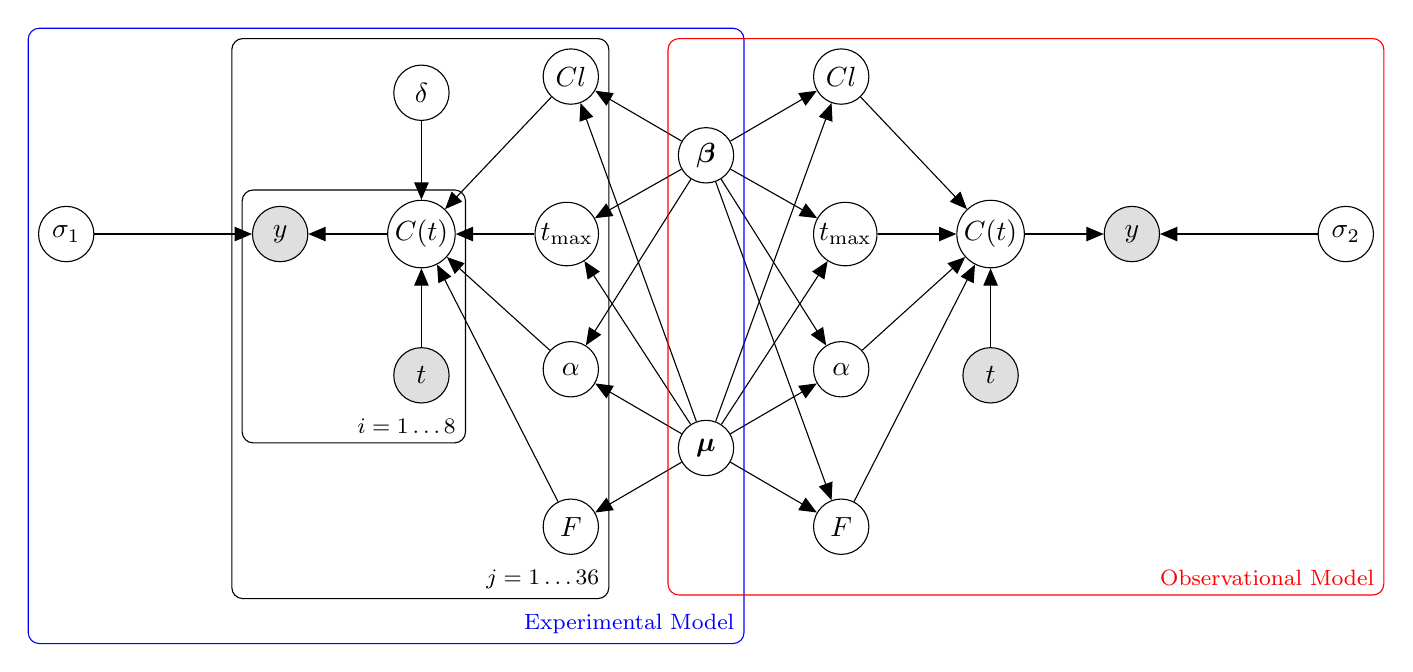
\begin{tikzpicture}
	\node[latent](b){$\boldsymbol{\beta}$};
	\node[latent, below= of b, yshift=-2cm](mu){$\boldsymbol{\mu}$};
	
	\node[latent, left= of b, yshift=1cm](r_Cl){$Cl$};
	\node[latent, left= of b, yshift=-1cm](r_t){$t_{\max}$};
	\node[latent, left= of mu, yshift=1cm](r_a){$\alpha$};
	\node[latent, left=of mu, yshift=-1cm](r_F){$F$};
	
	\edge{b}{r_Cl};
	\edge{b}{r_t};
	\edge{b}{r_a};
	\edge{mu}{r_Cl};
	\edge{mu}{r_t};
	\edge{mu}{r_a};
	\edge{mu}{r_F};

   	\node[latent, left= of r_t](r_C){$C(t)$};
   	
   	\edge{r_Cl}{r_C};
   	\edge{r_t}{r_C};
   	\edge{r_a}{r_C};
     \edge{r_F}{r_C};
   	
   	
   	\node[obs, left= of r_C](r_y){$y$};
   	\node[obs, below= of r_C](r_time){$t$};
   	\node[latent, above=of r_C](delay){$ \delta $};
   	
   	\edge{r_time}{r_C};
   	 \edge{delay}{r_C};
   	\edge{r_C}{r_y};
   	
   	\node[latent, left= of r_y, xshift=-1cm](r_sigma){$\sigma_1$};
   	
   	\edge{r_sigma}{r_y};
   	
	\plate[]{t_y_pairs}{(r_time)(r_y)(r_C)}{$i=1\dots8$};
	\plate{rommel_model}{(t_y_pairs)(r_C)(r_Cl)(r_t)(r_a)(r_F)}{$j = 1\dots 36$};

	
	\node[latent, right= of b, yshift=1cm](u_Cl){$Cl$};
	\node[latent, right= of b, yshift=-1cm](u_t){$t_{\max}$};
	\node[latent, right= of mu, yshift=1cm](u_a){$\alpha$};
	\node[latent, right= of mu, yshift=-1cm](u_F){$F$};
		
	\edge{b}{u_Cl};
	\edge{b}{u_t};
	\edge{b}{u_a};
	\edge{b}{u_F};
	\edge{mu}{u_Cl};
	\edge{mu}{u_t};
	\edge{mu}{u_a};
   \edge{mu}{u_F};
	

	\node[latent, right= of u_t](u_C){$C(t)$};
	
	  \edge{u_Cl}{u_C};
	\edge{u_t}{u_C};
	\edge{u_a}{u_C};
	\edge{u_F}{u_C};
	
	\node[obs, right= of u_C](u_y){$y$};
		
	\node[obs, below= of u_C](u_time){$t$};
	\node[latent, right= of u_y, xshift=1cm](u_sigma){$\sigma_2$};
	
	\edge{u_time}{u_C};
	\edge{u_C}{u_y};
	\edge{u_sigma}{u_y};
	
	\plate[color=blue]{experimental}{(b)(mu)(rommel_model)(r_sigma)}{\color{blue}{Experimental Model}};
	\plate[color=red]{observational}{(b)(mu)(u_Cl)(u_t)(u_a)(u_F)(u_C)(u_time)(u_y)(u_sigma)}{\color{red}{Observational Model}};
	\end{tikzpicture}

\end{figure}


\end{document}